%%% maw.tex
%% \section{Minimal Absent Words and Maximal Repeats}
\section{Minimal Rare Words and Maximal Repeats}
\label{sec:mrep}

%% We introduce a fundamental concept of maximal repeats of a string $S$, which is useful for realizing efficient enumeration of many kinds of unusual words. Then, we give a characterization of the set $\MRW(S)$ of minimal rare words of a string $S$.
%% 

% of the string $S = \texttt{aabaababb}$ are shown in \cref{fig:example:maw}. 


%% \mysubsubsection[]{Minimal rare words}
%% %%%% 
%% (MRW, for short) of a string $S$ are a class of unusual words, introduced by
%% Belazzougui and Cunial~\cite{belazzougui2015space:unusual}
%% %% Garcia, Pinho, Rodrigues, Bastos, and Ferreira~\cite{garcia2011minimal}.
%% A \textit{MRW} is a non-trivial string $w$ that does not occur in $S$, and any proper factor of $w$ occurs in $S$ as a substring (see \cite{garcia2011minimal}).
%% Precisely, a MRW of $S$ is a string $a u b$ with $a, b\in \hat\Sigma$ and $u \in \Sigma^+$ such that
%% \begin{enumerate*}[(i)]
%% \item $w \not\in \Fac(\hat S)$; and 
%% \item $au, ub \in \Fac(\hat S)$. 
%% \end{enumerate*}

%% \mysubsubsection[]{Minimal absent words}
%% %%%% 
%% %A \textit{minimal absent word} (MRW)
%% of a string $S$ are a class of unusual words, introduced by Garcia, Pinho, Rodrigues, Bastos, and Ferreira~\cite{garcia2011minimal}. A \textit{MRW} is a non-trivial string $w$ that does not occur in $S$, and any proper factor of $w$ occurs in $S$ as a substring (see \cite{garcia2011minimal}).
%% Precisely, a MRW of $S$ is a string $a u b$ with $a, b\in \hat\Sigma$ and $u \in \Sigma^+$ such that
%% \begin{enumerate*}[(i)]
%% \item $w \not\in \Fac(\hat S)$; and 
%% \item $au, ub \in \Fac(\hat S)$. 
%% \end{enumerate*}

%% As an example, the minimal absent words of the string $S = \texttt{aabaababb}$ are shown in \cref{fig:example:maw}. 

%%%%%%
%% \begin{algorithm}[t]
%% \centering  
%% %% 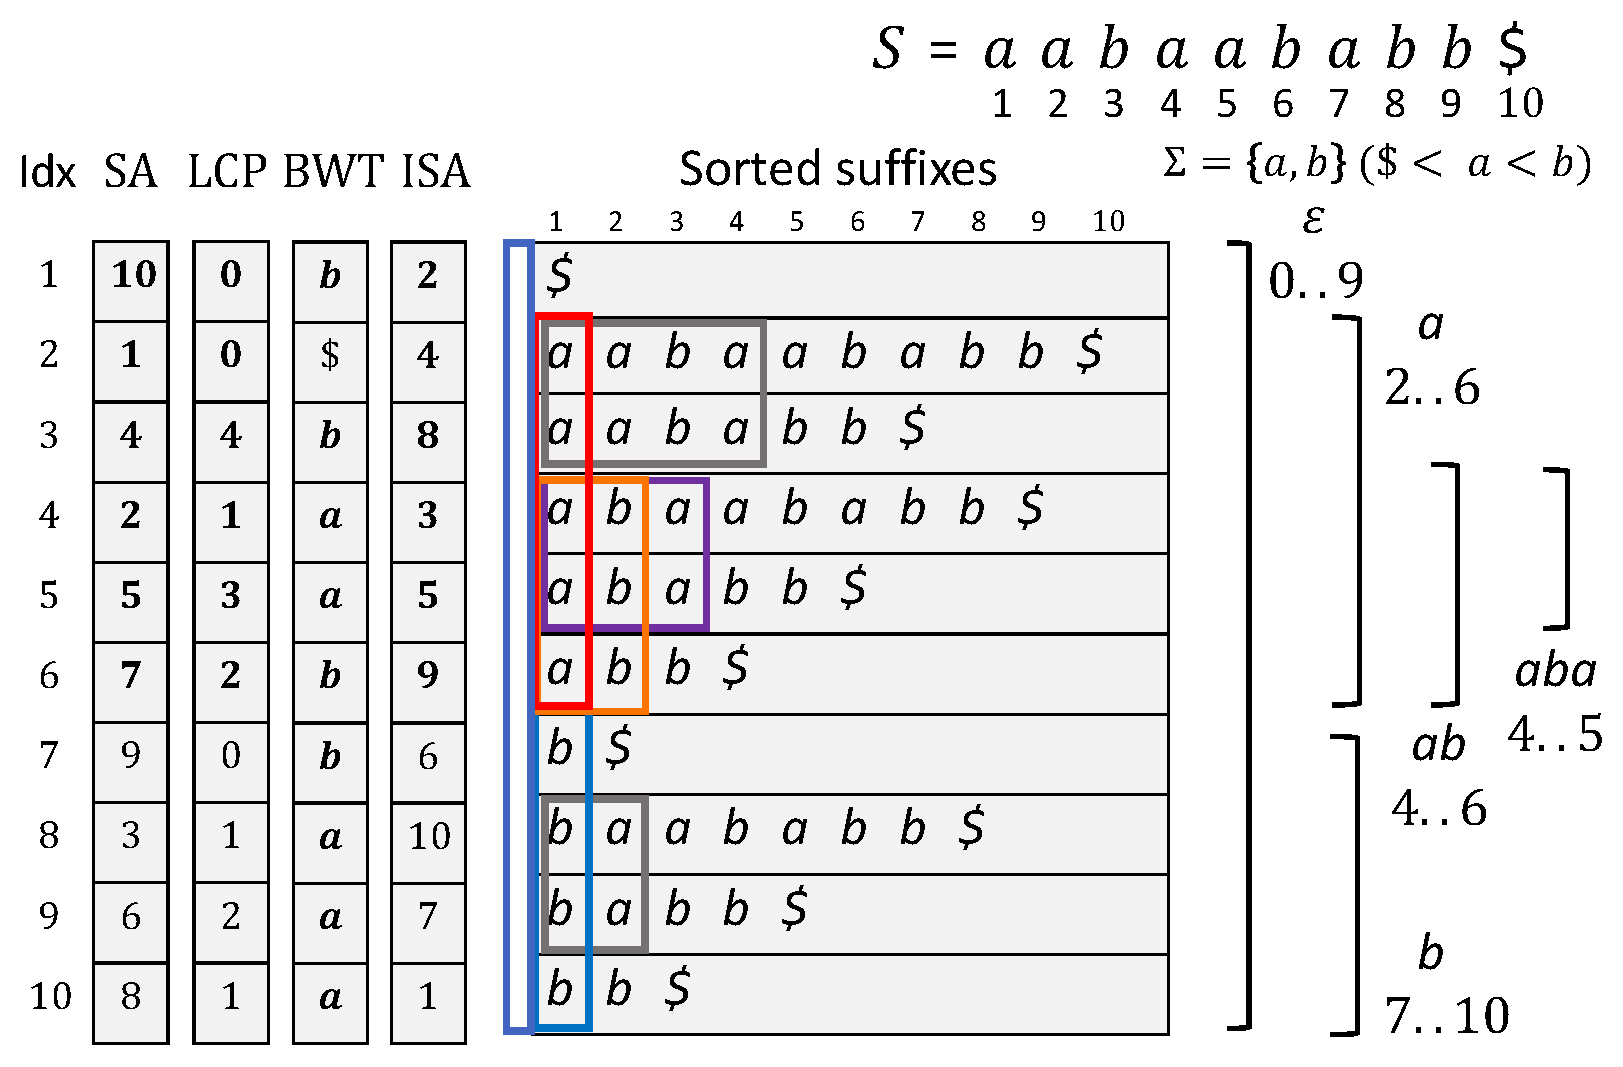
\includegraphics[width=0.60\textwidth]{fig/exp1/fig1.pdf}
%% \vspace{.5\baselineskip}
  %% \setlength{\interspacetitleruled}{0pt}%
%% \setlength{\algotitleheightrule}{0pt}%


%% %%%%%%
%% \begin{figure}[t]
%% \centering  
%% %% 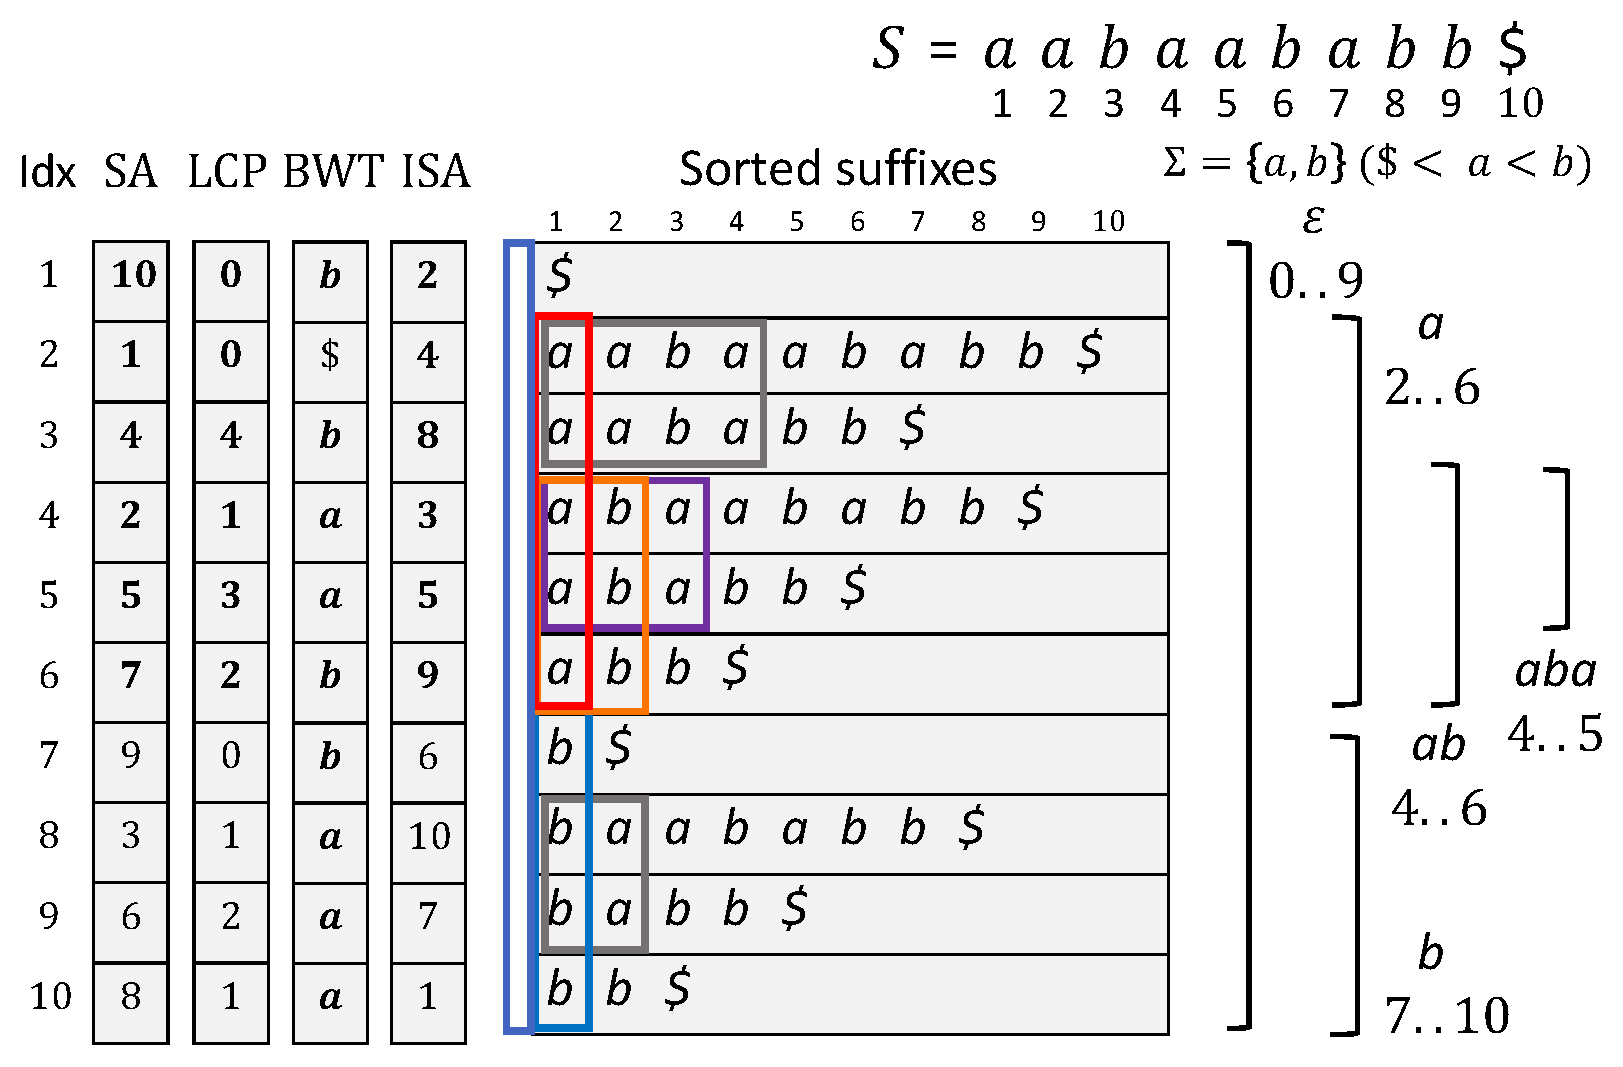
\includegraphics[width=0.60\textwidth]{fig/exp1/fig1.pdf}
%% \vspace{.5\baselineskip}
%% \caption{An example of minimal absent words of the string $S = \texttt{aabaababb}$. 
%% }\label{fig:example:maw}
%% \end{figure}
%% %%%%%%
%% %%%%%%%%%%%%%%%%%
%% \bgroup
%% {
%%   \setlength{\interspacetitleruled}{0pt}%
%%   \setlength{\algotitleheightrule}{0pt}%  
%%   \begin{algorithm}[h]
%%   %% \caption{Top-down MR-enumeration algorithm with \SA}\label{algo:maxrep:tdfw}
%%   \textbf{Procedure} \MRRec$(\tau_0 = ([L_0..R_0], \ell_0))$:\\
%%   %%\KwGiven{}
%%   %% \KwIn{The triple $\tau_0 = (L_0, R_0, \ell_0)$ for a right-branching substring $X$ of a string.}
%%   %% \KwOut{}
%%   \Begin{
%%       \textbf{output} $\tau_0$
%%       \Comment*{A maximal repeat is found}
%%       \For %(\CM{})
%%            {child $\tau = ([L..R], \ell)$ of the parent $([L_0..R_0], \ell_0)$}{
%%           \Comment{It is ensured that $R - L \ge 1$ and $\tau$ is right-branching}
%%           Decide if $\tau$ is left-branching by $\SA, \ISA$, and $S$ (\cref{lem:leftmaximal:character})\; 
%%           \If {$\tau$ is left-branching}{          
%%             \MRRec$(\tau)$\; 
%%           }
%%         }
%%   }
%%   \end{algorithm}
%% \egroup
%% %%%%%%%%%%%%%%%%%



%%% EOF
